\section{Introduction}
\label{sec:introduction}

%Context
Today's large scale internet services (e.g. Google Maps, Facebook, 
Amazon, etc.) handle millions of client requests, producing 
terabytes of data on a daily basis~\cite{parikh:facebook}. To handle 
this load, major internet companies have developed distributed 
databases called KV-stores such as Google's BigTable\cite{chang:bigtable},
Amazon's Dynamo~\cite{decandia:dynamo}, Yahoo's
PNUTS~\cite{cooper:pnuts}, Apache's HBase~\cite{george:hbase} and
Cassandra~\cite{hewitt:cassandra} (originally Facebook).

KV-stores are highly available to the user and provide advanced 
features like automated load balancing and fault tolerance. KV-stores 
scale horizontally -- by partitioning data and request load across a 
configurable number of nodes. To achieve these properties at a large-scale, 
KV-stores sacrifice an expressive query language and data model, only 
offering a simple API, comprising of \textit{put}, \textit{get} and 
\textit{delete} operations. While this API provides efficient access 
to single row entries, the processing of more complex (SQL-like) queries, e.g. 
selection, aggregation, and join, require costly application-level 
operations. Although, some KV-stores provide additional features to 
support higher-level query processing, those features are often 
rudimentary and impose bottlenecks. 

 Many existing approaches separate transactional and analytical 
processing. A complete snapshot of the data base is copied or loaded to 
an \textit{external} data warehouse and then, processed in a batch-wise 
fashion. Therefore, numerous existing frameworks with varying 
abstraction levels are available, e.g. Map Reduce \cite{dean:mapreduce}, 
Apache Spark \cite{zaharia:spark}, Apache Hive \cite{thusoo:hive}, etc. 
While this approach exploits the benefits of high performance parallel 
processing, it always requires an initial load overhead. Further it is 
not capable of providing up-to-date results -- as frequent changes in 
the base data occur. 

Another way of solving the problem is the use of \textit{internal} 
KV-store mechanisms that directly operate on the KV-store data. Apache 
Pheonix \cite{phoenix:apache} enables rich SQL 
semantics by using the coprocessor functionality (little code snippets, 
deployed on the KV-store nodes) of HBase. While this approach is 
implementation bound to a specific KV-store, we strive for a more general 
solution. 
 

Our approach introduces mechanisms for the materialization and 
incremental maintenance of views to KV-stores. The user 
attains sophisticated query capabilities, simply through definition of 
view expressions. The KV-store keeps results highly available and
enables access of many clients in parallel -- as materialized views 
are simple tables managed in KV-store. Likewise, views can be maintained 
incrementally; only those view records are updated whose 
base records have been changed. The challenge then, is not the scanning
 and computation of base data any more, but the efficient and correct 
maintenance of views. To achieve this at scale, we develop the 
\textit{Distributed View Maintenance System} (VMS) as shown in 
Figure~\ref{fig:research_goal}. The VMS consumes streams of client 
operations (of a base table) and produces the corresponding updates 
(to the view table). 

\begin{figure} 
	\centering 
	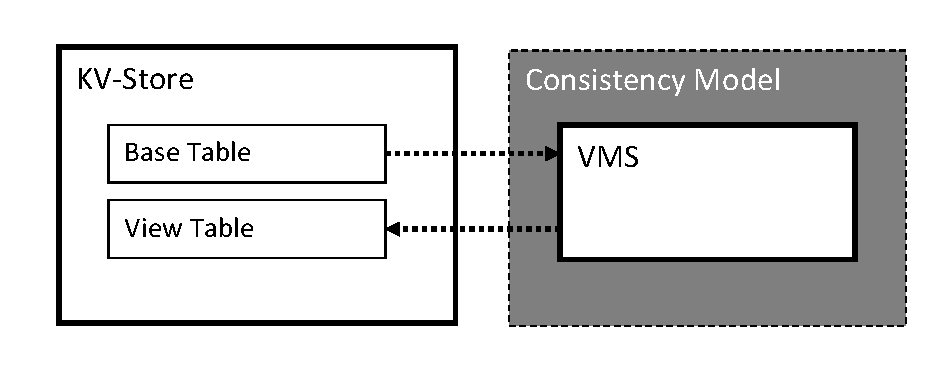
\includegraphics[width=\linewidth]{figures/ResearchGoal} 
	\vspace{-10mm} 
	\caption{System overview} 
	\vspace{-5mm} \label{fig:research_goal} 
\end{figure} 

First, we examine a set of KV-store 
implementations\cite{george:hbase, 
hewitt:cassandra, chang:bigtable, cooper:pnuts} and derive the common 
key characteristics from their architectures and their data models 
(Section~\ref{sec:kv_model}). As is common in the literature on view 
maintenance, we use a consistency model 
(Section~\ref{sec:consistency}) to ensure materialized views remain 
consistent with base data. But unlike the existing 
models\cite{zhuge:view, wang:efficient, zhang:parallel} -- which where 
mainly applied to centralized data warehouse environments -- we design 
our own consistency model to match the needs of a highly distributed 
environment (i.e. KV-stores). Based on the KV-store model and the requirements
of the consistency model, we describe 
the design of the scalable VMS (Section~\ref{sec:view_maintenance_system}). 
We design our VMS to scale in view update load and number of views 
maintained. Our design does not interfere with the read/write processing 
against tables in the KV-store, thus, leaving base table processing 
latencies unaffected. Finally, we conduct a comprehensive 
experimental study (Section~\ref{sec:evaluation}).

